\documentclass[12pt]{article}
\usepackage[margin=2.5cm]{geometry}
\usepackage{amsmath}
\usepackage{amssymb}
\usepackage{mathtools}  
\usepackage{diffcoeff}  
\usepackage{siunitx}
\usepackage[table,xcdraw]{xcolor}
\usepackage{amsfonts}
\usepackage{subfiles}
\usepackage{hyperref}
\usepackage{newtxtext, newtxmath}
\usepackage{enumitem}
\usepackage{titling}
\usepackage{listings}
\usepackage{float}
\usepackage{hyperref}
\setlength{\droptitle}{-6em}
\usepackage{placeins}
\usepackage{graphicx}
\usepackage{subcaption}
\usepackage[utf8]{inputenc}
\usepackage{fancyhdr}
\usepackage{color}
\usepackage{xspace}
\usepackage{pifont}

%%% This is about changing the headers and footers (i.e. Top and bottom of the page)
\pagestyle{fancy}% use fancyheaders with the bar on the top
\fancyhf{} % Clear the normal style
\fancyhead[L]{\bfseries\leftmark} %this places the section number and name in the top left
\fancyhead[R]{\bfseries\thepage}% this places the pagenumber in the top right
%%%% Add the bibliography with some settings:
% package:
% \usepackage[square, comma, numbers, sort&compress ]{natbib}
\usepackage[style=apa]{biblatex}
% bibliography sort style:

%%%%% frontmatter/mainmatter/backmatter:
\newcommand\frontmatter{%
    \cleardoublepage
    \pagenumbering{roman}} %small Roman numbers

\newcommand\mainmatter{%
    \cleardoublepage
    \pagenumbering{arabic}} %normal numbers

\newcommand\backmatter{%
    \cleardoublepage %% double page style
    %\clearpage %% single page style
    \pagenumbering{Roman}} %capital Roman numbers



\begin{document}
\newgeometry{margin=1.5cm} %% Special margins on the titlepage. It is also possible to set each margin separately; see package Geometry.
%%% Titelpagina in een apart bestand

\begin{titlepage} %%% This is your titlepage. Everything should match the conditions as they are right now for a physics thesis; hopefully the conditions won't change soon. In order to change this page into your very own title page, replace the noted parts with your own (like 'Your title').
	\noindent
	% \begin{minipage}{0.4\textwidth}
	% 	\includegraphics[width=\linewidth]{uulogo} %%%% Logo of the UU. English version is also available
	% \end{minipage}

    \par\vspace{1cm}
    
    \begin{flushright}
    {\LARGE\bfseries Utrecht University \par} %Enter your faculty here. It is probably right already (usually in Dutch).
    \end{flushright}
	\vspace{1cm}
    \begin{center}
    {\huge\bfseries Emulating SAI Scenarios in CESM2 and the Effects on the High-Latitude Southern Hemisphere Atmospheric Circulation\par} %% ENTER TITLE HERE
    \end{center}
	\vspace{1cm}
    {\scshape\Large Master Thesis\par}
	\vspace{0.5cm} % You change this to set the distance 'Bachelor Thesis' to 'Your name', and all the other vspaces to set the heights of everything.
	{\Large\itshape Simone Lingbeek\par} %% ENTER NAME HERE
    \vspace{0.5cm}
    % \centering
    % \fbox{ %% fbox puts a black border around your picture
    % \includegraphics[height=0.35\textheight]{Clipboard01} %% If you use a picture, place it here. If you don't, delete this, from '\centering' to '\par'.
    % %% change the height ration until it fits.
    % } %% the fbox ends here
    % \vspace{0.5cm}
    % \par
    \raggedleft
	{\Large\itshape Supervisors}:\par\vspace{0.25cm}
	{\large Dr. Claudia Wieners \textsc{Supervisor}\par} %% first supervisor
    Institute for Marine and Atmospheric research Utrecht\par %% their institute
    \vspace{0.25cm}
    {\large Dr. Michiel Baatsen \textsc{Supervisor}\par} %%second supervisor
    Institute for Marine and Atmospheric research Utrecht\par %% their institute
    \vspace{0.25cm}
    {\large Jasper de Jong \textsc{Daily supervisor}\par} %%daily supervisor
    Institute for Marine and Atmospheric research Utrecht %% their institute
    %% copy/paste from \vspace{0.25cm} to here for more supervisors.

	\vfill
	{\large \today\par}%%% The date. Replace \today with the necessary date if your necessary date isn't today.
    
\end{titlepage}    

\restoregeometry %%% Restores the margins for the rest of the document.


\section{Introduction}
\subsection{Climate change and geoengineering}
In the effort of limiting the effects global climate change, eliminating fossil fuels is the most important step to take. Regrettably, the complete elimination of fossil fuels in time to prevent the most disastrous effects of climate change and limit global warming to even 2°C is becoming increasingly unlikely. Even with all currently committed climate action goals, projections show the earth warming significantly above the 1.5°C and 2°C targets from the Paris Agreement \parencite{NDCsynth}. With this outlook, methods to temporarily lower the earth's global temperature are looked at to buy the global community time to lower atmospheric greenhouse gases. One such method is solar radiation management with stratospheric aerosol injections (SAI). 

Geoengineering can be seen as a toolbox of methods that change the earth's climate system to achieve a desired effect. Limiting global mean surface temperature (GMST) increase is the primary goal of geoengineering. The methods of geoengineering can be divided into two basic categories, Carbon Dioxide Removal (CDR) and Solar Radiation Management (SRM) \parencite{shepherd2009}. CDR focuses on lowering the amount of greenhouse gases in the atmosphere, by capturing CO$_2$ directly or enhancing and facilitating natural processes to speed up the extraction of CO$_2$ from the atmosphere or oceans. SRM on the other hand focuses on altering the earth's radiation budget. This can be done by increasing the amount of long wave radiation the earth emits into space, for instance with cirrus cloud thinning, but the most widely discussed approach is increasing how much short wave radiation from the sun is reflected back into space, i.e. increasing the planetary albedo. This is done for instance by making deserts more reflective or making clouds brighter like through marine cloud brightening \parencite{reflecting}. 

\subsection{Geoengineering in the Form of Stratospheric Aerosol Injections}
This thesis considers SRM in the form of stratospheric aerosol injections (SAI). Through injection of sulphate aerosols or their precursors at specific points in the stratosphere the earth's radiation budget is changed. At this high altitude the aerosols reflect short wave radiation, lowering the amount of sunlight reaching the earth's surface and subsequently GMST is lowered. It has been argued that SAI is one of the most feasible options for SRM \parencite{lenton2009,shepherd2009}.

A direct result of SAI is the absorption of long wave radiation emitted by the earth by the aerosols, resulting in warming in the stratosphere \parencite{Ammann2010}. This impacts the global atmospheric circulation patterns and precipitation patterns. It is also important to keep in mind that the effects other than warming caused by increased greenhouse gases are still present in the earth system, for instance ocean acidification will continue if CO$_2$ concentrations continue to rise. The introduction of sulphate aerosols has unintended consequences too, including in delayed repair of the ozone hole and an increase in acid deposition, and interference with cloud formation. 

Eventhough complete understanding of the physical consequences of SAI is not within reach as of now, the physical feasibility in regards to limiting global warming is rather certain. Practically, the succesful deployment of SAI is only possible if the global community can reach consensus on its employment and can ensure no party deploys SAI undemocratically and to the detriment of others. Even then, long-term political and economical stability are crucial, as an abrupt halt would lead to rapid warming \parencite{robock2009}. 

The employment of SAI is not as straight-forward as appears at first glance, and before any decisions can be made about SRM, with SAI or through other means, more research is needed. The National Academy of Sciences made extensive recommendations for solar geoengineering research \parencite{reflecting}, including research into the impacts on atmospheric processes, the climate response, desigining a monitoring system, how to govern solar geoengineering activities and ethical considerations for current and future generations. 

\subsection{General Structure}
In this thesis we investigate the climate response to SAI, more specifically the atmospheric dynamics of the Southern Hemisphere. We will use the results from a previous study on SAI conducted with an earth system model with an extensive atmospheric component and comprehensive atmospheric chemistry to build an emulator with a model with a smaller atmospheric component that incorporates no atmospheric chemistry. We do this primarily to save on computation time. We will validate this experiment in Part I, and use it to assess the impact of SAI on the Southern Hemisphere atmospheric circulation in Part II. We will focus on changes in the large scale components of the atmospheric circulation. 

The southern hemisphere is of particular interest because of the Antarctic Ice Sheet that is home to a number of tipping points. The triggering of these tipping points can potentially lead to disastrous levels of sea level rise and once these tipping points are reached, there is no way to reverse the effects. Understanding the dynamics of the Southern Hemisphere and the response to SAI is crucial to accurately predict the future evolution of these tipping points and if triggering them can be avoided with the help of SAI. 

\newpage
\section{Introduction Part I}
\subsection{Previous Research on SAI in Earth System Models}
Large scale studies on SRM started with the Geoengineering Model Intercomparison Project (GeoMIP) \parencite{geomip2011}. Experiments reduced the incoming solar radiation either directly or through injection of SO$_2$ in the stratosphere at one point on the equator, which was then distributed in the atmosphere very quickly by the zonal circulation and on larger time scales the meridional circulation.

It was found that injection of aerosols at just the equator, and uniform solar radiation reduction lead to over-cooling of the tropics and under-cooling of the poles. \textcite{kravitz2016} proposed a different approach, where climate targets were considered the main goal and how to reach those goals through SAI was viewed as a design problem. One set of targets proposed was the global mean surface temperature ($T_0$), the interhemispheric temperature gradient ($T_1$) and the pole-to-equator temperature gradient ($T_2$). The proposed SAI strategy included four injection points, two on each hemisphere, and a feedback algorithm that adjusts the injection rate at those points to achieve the temperature goals. This method was applied by \textcite{kravitz2017} and \textcite{macmartin2017}, and then in the Geoengineering Large Ensemble (GLENS) project \parencite{tilmes2018}. 

\subsection{The GLENS Project and Subsequent CESM2 Simulations}
The GLENS project is a 20-member ensemble of gradual SAI simulations. From 2020 onwards SO$_2$ is injected at four injection points at $\pm$ 15°N and $\pm$ 30°N about 5 km above the tropopause. A feedback-control algorithm is used to adjust the injection amounts at each point individually based on the departure of the $T_{0,1,2}$ temperatures defined by \textcite{kravitz2016} from 2020 levels.

The GLENS project was performed using the Community Earth System Model version 1 (CESM1) \parencite{hurrell2013}, with the Whole Atmosphere Community Climate Model (WACCM) as its atmosphere component. This model uses a 0.9° latitude $\times$ 1.25° longitude rectangular grid with 70 vertical layers that reach up to 140 km, or about 10$^{-6}$ hPa. It includes comprehensive atmospheric chemistry for the middle atmosphere, incorporating ozone chemistry and chemistry relating to stratospheric sulfate formation. A simpler chemistry scheme is used for the troposphere. Aerosol chemistry is coupled to WACCM through the three-mode version of the Modal Aerosol Module (MAM3).

After the GLENS project the method using four injection points and a feedback algorithm was further explored using the more recent Community Earth System Model version 2, also using a newer version of the WACCM, now version 6 (CESM2(WACCM6)) \parencite{tilmes2020}. WACCM6 has the same horizontal and vertical resolution, but now includes comprehensive chemistry from the troposphere up to the lower thermosphere. The MAM4 modal aerosol scheme is used for the troposphere and stratosphere. We will refer to this model as `WACCM'.

Because WACCM is comprehensive in both vertical resolution and atmospheric chemistry, it is well-suited to simulate SAI scenarios. However, due to this it is also a very cumbersome model, requiring more computing time and resources compared to less comprehensive models. This limits its use in ensemble studies and studies considering a large range of scenarios. Computational cost also limits its use for simulations with a longer timeseries at higher resolution, required to study smaller scale phenomena like tropical cyclones. 

\subsection{Building an Emulator for SAI with CESM2(CAM6)}
Reducing the amount of computing resources needed for an experiment can be done by using a smaller, less comprehensive model and using previous results from WACCM as external forcing to the model, essentially building an emulator. \textcite{pfluger2024} introduce a method for building such an emulator of WACCM to model SAI. They use the same CESM2 model configuration is used as in \textcite{tilmes2020}, but the Community Atmosphere Model version 6 (CAM6) is used for the atmosphere component \parencite{danabasoglu2020}. This model has only 32 vertical levels and no atmospheric chemistry. We will refer to this model as `CAM'. The aerosol field established in the WACCM simulation is used as an external forcing. To maintain 2020 levels of GMST, the necessary globally averaged aerosol optical depth (AOD) field is found though the same feedforward-feedback algorithm. All other forcing fields are then scaled accordingly. In contrast to the WACCM simulations, the temperature gradients $T_1$ and $T_2$ are not adjusted for. 

The WACCM SAI experiment is well-suited to build an emulator for, as the employment of SAI is used as a means to reach a climatic goal. It prescribes an aerosol burden in response to model behaviour, in stead of gauging the model response to a certain aerosol burden. This removes the amount of SO$_2$ injected into the stratosphere from the experiment design and allows for translation of the aerosol distribution to another model that might respond differently to the introduction of aerosols.

\subsection{Scenarios Part I}
There are two simulations performed with CAM and WACCM. The first simulation follows the historical spin-up and is continued by the SSP5-8.5 scenario \parencite{RIAHI2007887}. The second simulation branches from the first simulation in 2020 and from then on introduces SAI to stabilise temperatures using the SSP5-8.5 scenario as background. Here we will refer to it as the gradual SAI scenario. A schematic view of the GMST response in each scenario is shown in Figure \ref{fig:schematic_scens_pt1}.

\begin{figure}[H]
    \centering
    \includegraphics[width=0.6\linewidth]{images/schematic_scens_pt1.png}
    \caption{Schematic of the global mean surface temperature in the two scenarios used in Part I, the SSP5-8.5 and gradual SAI scenarios.}    
    \label{fig:schematic_scens_pt1}
\end{figure}


\newpage
\subsection{Research Questions Part I}
The fist part of this thesis is the validation of this method and model in its use as an emulator, simulating SAI scenarios based on the WACCM results. Two experiments, a high-warming scenario and a gradual SAI scenario, are used to assess the impact of SAI in each model (CAM and WACCM). We calculate the three temperature targets for all models and we will look at the model results for 2-meter temperature for additional insight into the performance of CAM in regards to regulating surface temperatures. We discuss both annual and seasonal patterns. Additionally, we discuss precipitation patterns.

The most important difference in dynamics between the two models lies in the inclusion of ozone chemistry and thus the interaction of stratospheric aerosols and ozone. It is known that sulphate aerosols in the stratosphere accelerate chemical ozone loss through halogen activation and strengthening of the polar vortex \parencite{bednarz2023ozone}. CAM does not include this process, and assessing whether the dynamical response to SAI is comparable to WACCM is thus important. To this end we assess any differences in the vertical profile between the two models, we compare the zonally averaged potential temperature and zonal winds. 

We formulate the following research questions for Part I:
\newline

\noindent \textit{When applying the stratospheric aerosol emulator to a gradual SAI scenario in CESM2(CAM6), are we able to reproduce from \textcite{tilmes2020}
    \begin{enumerate}[label=\roman*]
        \item the temperature targets $T_0$, $T_1$ and $T_2$?
        \item the spatial and seasonal variations of temperature, precipitation and general aspects of the atmospheric circulation?
    \end{enumerate}
}

\subsection{Results SAI in WACCM}
The experiments performed with WACCM \parencite{tilmes2020} showed that surface temperatures were generally controlled with SAI. Under SAI the tropics warmed slightly, the mid-latitudes cooled slightly and the poles warmed slightly as well. Zonal mean precipitation showed an increase in the tropics and a decrease or no significant change everywhere else. An apparent warming hole over the Northern Atlantic was observed in all simulations and was likely related to observed changes in the Atlantic Meridional Overturning Circulation. No changes in seasonal patterns were discussed, nor were changes in potential temperature and atmospheric circulation. 


\newpage
\section{Introduction Part II}
\subsection{Rapid Cooling with SAI as an Emeregency Intervention}
As sufficient climate policies to prevent global warming of 1.5°C or even 2°C \parencite{NDCsynth}, it is unlikely the global community will implement a proactive gradual SAI scenario in time as well. Employing SAI much later on after prolonged heating of the climate system is a realistic, more reactive, scenario. The earth could be cooled very rapidly, allowing the end-of-century GMST goals to be reached after the climate system has endured an even longer period of warming than it has to date. The effects of such an intervention are largely uncertain. While it is rather certain that SAI could lower GMST, it is not certain what effects of previous warming can be reversed, if at all. The SAI 2080 scenario introduced in \textcite{pfluger2024} is such a scenario, SAI is employed from 2080 onwards to achieve rapid cooling to 2020 levels. 

\subsection{Scenarios Part II}
For the second part of this thesis we consider the two CAM simulations from Part I, the SSP5-8.5 and the gradual SAI simulations, and the SAI 2080 scenario from \textcite{pfluger2024}. We will refer to this simulation as the rapid cooling SAI simulation. The rapid cooling simulation is branched from the SSP5-8.5 simulation in 2080, SAI is then deployed to restore $T_0$ to 2020 levels. The control algorithm is adjusted up to the first six years to prevent extremely high aerosol concentrations that would result in too rapid cooling. A schematic view of the GMST response for this scenario is shown in Figure \ref{fig:schematic_scens}.

\begin{figure}[H]
    \centering
    \includegraphics[width=0.65\linewidth]{images/schematic_scens.png}
    \caption{Schematic of the global mean surface temperature in the two scenarios used in Part I, the SSP5-8.5, the gradual SAI and the rapid cooling SAI scenarios.}  
    \label{fig:schematic_scens}  
\end{figure}


\subsection{The Southern Hemisphere Atmopshere}
The atmosphere is home to a number of large scale circulation phenomena. Though the two hemispheres are symmetrical in the occurence of these phenomena, the exact location, frequency of occurence and other behaviour of these phenomena differs between the two hemispheres. The Southern Hemisphere circulation is generally more stable than its counterpart in the Northern Hemisphere. In this thesis we focus on three so-called jets, large scale circulation phenomena that persist throughout the year or in a specific season.
We discuss the subtropical jet and the the eddy-driven jet in the lower stratosphere (up to 50 hPa), and the polar night jet in the upper stratosphere (above 50 hPa).


\subsubsection{The Subtropical Jet}
The subtropical jet (STJ) forms at the convergence of the upper branches of the Hadley and Ferrel cells in the lower stratosphere, with a maximum around 200 hPa, see Figure \ref{fig:jetcrosssection} (the Southern Hemisphere is analogous to the Northern Hemisphere). Influenced by the Coriolis force westerly winds form here, the magnitude of which is determined by the temperature gradient below the convergence zone \parencite{zolotov2018variability}. The STJ occurs year-round but is strongest in winter, in tandem with the stronger winter Hadley cell, where it is located around 30°S.

In the past decades, the southern hemisphere STJ has been observed to shift poleward and slightl decrease in wind speed, though not significant \parencite{zolotov2018variability}. The STJ was also observed to be increasingly wavy \parencite{martin2023}. Under high global warming the STJ is projected to shift further poleward and increase in strength \parencite{chenoli2017historical}. 

Simulations with SAI at singular injection points showed a small but significant decrease in the strength of the STJ \parencite{richter2017}. From historical simulations it has been argued as well that anthropogenic aerosols contribute to deceleration \parencite{wang2020}.

\begin{figure}[t]
    \centering
    \includegraphics[width=0.8\linewidth]{images/Jetcrosssection.png}
    \caption{Cross section of the Northern Hemisphere atmospheric ciruclation, with the suptropical jet and polar jet (or eddy-driven jet) in relation to the circulation cells. Image by: Original: National Weather Service, JetStream Vector: Sleske - Own work based on: Jetcrosssection.jpg, CC BY-SA 4.0, \href{https://commons.wikimedia.org/w/index.php?curid=75169357}{https://commons.wikimedia.org/w/index.php?curid=75169357}}  
    \label{fig:jetcrosssection}  
\end{figure}


\subsubsection{The Eddy-driven Jet}
At the divergence of the upper branches of the Ferrel and Polar cells another jet forms, the polar jet in Figure \ref{fig:jetcrosssection}. This jet is at a lower altitude and stronger than the STJ. However, it is also much wavier than the STJ \parencite{martin2023}. Because of this, and to avoid confusion with the polar night jet, we will refer to this jet as the eddy-driven jet (EDJ). 

The EDJ has been observed to become increasingly wavy in the past decades, also shifting poleward, even more strongly than the STJ, but no significant trend in the wind speed was observed \parencite{martin2023}. Under high global warming the EDJ is projected to shift further poleward \parencite{Curtis_2020}.

It is not certain how the EDJ will respond under SAI, though it has been shown that the EDJ is influenced by the strength of the polar night jet in the upper stratosphere, where a strengthened jet leads to a poleward shift of the EDJ \parencite{kidston2015stratospheric}. Any changes in the polar night jet due to SAI are thus likely to cause changes in the EDJ as well.

\subsubsection{The Polar Night Jet}
The polar night jet (PNJ) forms in the upper stratosphere during winter in response to the large equator-to-pole meridional temperature gradient. The pole becomes encircled with a belt of strong westerly winds in the upper parts of the stratosphere, above $\approx$50 hPa at around 60°S \parencite{lee2021}. 

With high warming the PNJ is projected to increase in strength, most notably in late SH spring, effectively delaying the ultimate breakdown of the PNJ \parencite{ceppi2019}.

The warming in the lower stratosphere due to SAI leads to an increase of the equator-to-pole meridional temperature gradient, causing increasing zonal winds via the thermal wind balance. This effect is strongest in the late winter/early spring \parencite{bednarz2023injection,bednarz2023ozone}.

When disturbances near the surface propagate to the stratosphere, the PNJ can suddenly weaken, leading to a sudden increase in temperatures of the polar stratosphere and sometimes a complete breakdown of the jet. These events are called sudden stratospheric warming events (SSWs) and occur very rarely in the Southern Hemisphere in the current climate. Their frequency is projected to strongly decrease with increasing global warming \parencite{jucker2021}. 


\subsection{Antarctica and the Southern Hemisphere Atmosphere}
The high-latitude Southern Hemisphere is of particular interest in the context of climate change and the prevention of it. The Antarctic Ice Sheet (AIS) could contribute greatly to global sea level rise if it were to become unstable under global warming. Observed instabilities of the West-Antarctic Ice Sheet (WAIS) alone could contribute to significant sea level rise \parencite{IPCC_2021_WGI_Ch_9}. 

Large scale atmospheric dynamical changes affect the Antarctic ice sheet, changes in temperature, precipitation and wind fields alter the surface mass balance of the ice sheet. More distantly dynamical changes affect the ice sheet through changes in the ocean, mainly in the rate and location of overturning circulations. A warmer ocean together with a warmer atmosphere can lead to the loss of ice shelves \parencite{WANG2023} and their disappearance has been observed to increase the flow of glaciers feeding into the ocean \parencite{scambos2004}, contributing to mass loss of the AIS. 

The Southern Hemisphere high stratosphere has low variability in the current climate, but any changes could have far-reaching effects on the surface climate. It has been observed that SH stratospheric polar vortex weakekening contributes to climate anomalies in Australia and New Zealand, southeast Africa and southern South America. Additionally, the wind stress over the ocean around Antarctica is weakened and the Ross and Amundsen seas experience warmer climate \parencite{domeisen2020}. There is thus a clear interaction between the atmospheric dynamics and local climate in the Southern Hemisphere. 

The effect of SAI on the Antarctic ice sheet has been studied by \textcite{mccusker2015}, who found that a rapid introduction of sulphate aerosols in the stratosphere could not prevent the collapse of the WAIS. \textcite{sutter2023} found similar results. However, both studies use very simple aerosol schemes, that for instance only inject aerosols in the tropics. These types of schemes are known to lead to over-cooling of the tropics and under-cooling of the poles. As stated before, the studies using a feedback-control algorithm to maintain the $T_{0,1,2}$ temperature targets were laregely successful in this regard. 


\subsection{Research Questions Part II}
In the second part of this thesis the effect of SAI on the high-latitude Southern Hemisphere atmospheric dynamics is investigated, both in the gradual and rapid cooling scenarios. The focus here lies on large scale circulation patterns, as they largely dictate local climate in the Southern Hemisphere. 

We formulate the following research quesitons for Part II:
\newline

\noindent \textit{What are the impacts of the gradual SAI scenario on the Southern Hemisphere
    \begin{enumerate}[label=\roman*]
        \item subtropical and eddy-driven jets in the lower stratosphere?
        \item polar night jet and sudden stratospheric warming events in the upper stratosphere?
    \end{enumerate}
How do the results for i and ii change under the rapid cooling SAI scenario?
}
\newpage

\part{Model Validation}
\section{Introduction Part I}
\subsection{Geoengineering in the Form of Stratospheric Aerosol Injections}
Geoengineering can be seen as a toolbox of methods that change the earth's climate system to achieve a desired effect. Limiting global warming to 1.5-2°C is the primary goal of geoengineering. The methods of geoengineering can be divided into two basic categories, Carbon Dioxide Removal (CDR) and Solar Radiation Management (SRM) \parencite{shepherd2009}. CDR focuses on lowering the amount of greenhouse gases in the atmosphere, by capturing CO$_2$ directly or enhancing and facilitating natural processes to speed up the extraction of CO$_2$ from the atmosphere or oceans. SRM on the other hand focuses on altering the earth's radiation budget. This can be done by increasing the amount of long wave radiation the earth emits into space. The most widely discussed approach is increasing how much short wave radiation from the sun is reflected back into space, i.e. increasing the planetary albedo. This is done for instance by making deserts more reflective or making clouds brighter. 

This thesis deals with SRM in the form of stratospheric aerosol injections (SAI). Aerosols or their precursors, in this case SO$_2$, are injected into the lower stratosphere where they reflect some of the incoming short wave radiation from the sun. This lowers the temperature of the earth's surface at the latitudes it was injected. As atmospheric circulation carries the aerosols around the globe zonally very quickly, only the latitude and season of the injection need to be considered. This choice was found to be crucial when determining the effectiveness of SAI on the poles by \textcite{duffey2023}. A more recent development in this regard started with \textcite{kravitz2017} and \textcite{macmartin2017}, and then the Geoengineering Large Ensemble (GLENS) project. 

\subsection{The GLENS Project and Subsequent CESM2 Simulations}
The GLENS project is a 20-member ensemble of gradual SAI simulations (Tilmes et al. 2018). From 2020 onwards SO$_2$ is injected at four injection points at $\pm$ 15°N and $\pm$ 30°N about 5 km above the tropopause. A feedback-control algorithm is used to adjust the injection amounts at each point individually based on departures from the temperature goals defined by \textcite{kravitz2016}. These are the global mean surface temperature, the inter-hemispheric temperature gradient and the equator-to-pole temperature gradient. This algorithm also tunes the injection amount to the seasonal response of the model. 

The GLENS project was performed using the Community Earth System Model version 1 (CESM1) \parencite{hurrell2013}, with the Whole Atmosphere Community Climate Model (WACCM) as its atmosphere component. This model uses a 0.9° latitude $\times$ 1.25° longitude rectangular grid with 70 vertical layers that reach up to 140 km, or about 10$^{-6}$ hPa. It includes comprehensive atmospheric chemistry for the middle atmosphere, incorporating ozone chemistry and chemistry relating to stratospheric sulfate formation. A simpler chemistry scheme is used for the troposphere. Aerosol chemistry is coupled to WACCM through the three-mode version of the Modal Aerosol Module (MAM3). \textcolor{teal}{past dit misschien beter in de methods, en dan voor cesm2?}

After the GLENS project the method using four injection points and a feedback algorithm was further explored using the more recent Community Earth System Model version 2, also using a newer version of the WACCM, now version 6 (CESM2(WACCM6)) \parencite{tilmes2020}. WACCM6 has the same horizontal and vertical resolution, but now includes comprehensive chemistry from the troposphere up to the lower thermosphere. The MAM4 modal aerosol scheme is used for the troposphere and stratosphere. \textcolor{teal}{dus dit ook naar methods? }

Because CESM2(WACCM) is so comprehensive in both vertical resolution and atmospheric chemistry, it is extremely well-suited to simulate SAI scenarios. However, due to this it is also a very cumbersome model, requiring a lot of computing time an resources. This limits its use in ensemble studies and studies considering a large number of scenarios. 

\subsection{CESM2 with CAM6 as an Emulator}
To reduce the amount of resources needed, \textcite{pfluger2024} introduce a method that uses a less comprehensive atmospheric component. The same CESM2 model configuration is used as in \textcite{tilmes2020}, but the Community Atmosphere Model version 6 (CAM6) is used for the atmosphere component \parencite{danabasoglu2020}. The aerosol field established in the CESM2(WACCM6) simulation is used as an external forcing. A feedforward-feedback algorithm is used to adjust the aerosol field as a whole to keep the global mean surface temperature (GMST) at 1.5°C above pre-industrial levels. So, in contrast to the CESM2(WACCM6) simulations, the temperature gradients are not adjusted for. 

To assess how well this method works as an emulator, the model results for surface temperature, precipitation, potential temperature and zonal wind are compared between CESM2(WACCM6) and CESM2(CAM6). \textcolor{teal}{dit mag uitgebreider}

To repeat, we formulate the following research questions:

\begin{enumerate}
    \item Does the CESM2(CAM6) succeed in maintaining global surface temperature through SAI, including spatial patterns?
    \item How does the CESM2(CAM6) SAI simulation perform compared to the CESM2(WACCM6) SAI simulation it was based on?
\end{enumerate}

The three temperature targets are calculated for all models. The model results for reference height temperature (or 2-meter temperature), will provide additional insight into the performance of CESM2(CAM6) in regards to regulating surface temperatures. Both annual and seasonal patterns are discussed. Additionally, precipitation patterns are discussed. To assess any differences in the vertical profile between the two models, the zonally averaged potential temperature and zonal winds are compared. 
\newpage

\section{Methods Part I}
\subsection{Building the Emulator for SAI simulations}
The emulator for SAI simulations is introduced in \textcite{pfluger2024}, it implements SAI via prescribed aerosol fields, as opposed to sulphate injections that result in aerosol fields through model physics. As per \textcite{pfluger2024}, the protocol works as follows:
\begin{itemize}
    \item Every year, observe the deviation of GMST from the target.
    \item Based on past GMST deviations, infer the level of SAI - expressed in terms of global mean aerosol optical depth (AOD) - which is necessary to achieve the desired target.
    \item Use the AOD to scale all SAI-related aerosol fields appropriately.
    \item Feed the scaled fields into CAM6.
\end{itemize}

The first two steps are implemented via the feedforward-feedback control algorithm as established in \textcite{kravitz2017}. The control algorithm stabilises only GMST, not inter-hemispheric and equator-to-pole temperature gradients like the simulation performed by \textcite{tilmes2020}.

The prescribed aerosol fields are the averaged aerosol fields from the WACCM simulation, this simulation is called the \textit{Geo SSP5-8.5 1.5 scenario} in \textcite{tilmes2020}. The fields are normalised, averaged and fit, to then arrive at an amplitude for each aersol component.

\textcolor{teal}{Stukje over aerosolveld hoe het eruit ziet + jaarlijkse totale massa figuren (?)}

\subsection{Definition of Scenarios and Time Periods for Part I}
There are two simulations performed with each CESM2 configuration. The first simulation follows the historical spin-up and is continued by the SSP5-8.5 scenario. The second simulation branches from the first simulation in 2020 and from then on introduces SAI to stabilise temperatures using the SSP5-8.5 scenario as background. Here we will refer to it as the gradual SAI scenario. 

Throughout this first part, three time periods are used to visualise and interpret the results from the simulations. For each period the 20-year mean is taken, unless specified otherwise. These periods are defined as follows:

\begin{itemize}
    \item \textbf{Reference} The period 2016-2035 of the SSP5-8.5 simulation.
    \item \textbf{Control} The period 2080-2099 of the SSP5-8.5 simulation.
    \item \textbf{SAI 2020} The period 2080-2099 of the gradual SAI simulation.
\end{itemize} 
\textcolor{teal}{misschien beter in tabelvorm}

\subsection{Vertical Interpolation}
The atmospheric vertical levels of CESM are defined as hybrid levels. However, for ease of computation and visualisation, conversion to pressure levels is preferred. To this end, a logarithmic interpolation scheme is used, that takes the model output at hybrid levels and projects them onto the appropriate pressure levels. For CAM the model output is converted to 34 pressure levels ranging from 3.5 to 993 hPa. For WACCM the SSP5-8.5 model output was pubplished in pressure levels, 19 pressure levels ranging from 1 to 1000 hPa. The WACCM gradual SAI scenario model output is converted to those same 19 pressure levels. \textcolor{teal}{moet dit uitgebreider?}

No interpolation is needed of the horizontal grids as these are identical in all models. 

\subsection{Temperature Targets}
The WACCM simulations use the feedback algorithm to maintain three temperature targets in their SAI scenario. These temperature targets are defined in \textcite{kravitz2016} as the projection of $T(\psi)$ onto the first three Legendre polynomial functions of $\sin(\psi)$, resulting in

\begin{equation}\label{eq:TdA}
    \begin{split}
        T_0 &= \frac{1}{A} \int\displaylimits_{-\pi/2}^{\pi/2} T(\psi) \mathop{dA},\\
        T_1 &= \frac{1}{A} \int\displaylimits_{-\pi/2}^{\pi/2} T(\psi) \sin(\psi) \mathop{dA,}\\
        T_2 &= \frac{1}{A} \int\displaylimits_{-\pi/2}^{\pi/2} T(\psi) \frac{1}{2}(2\sin^2(\psi) -1) \mathop{dA},
    \end{split}
\end{equation}

\noindent where $\psi$ is latitude, $T(\psi)$ is the zonal-mean temperature for each latitude, and A the area-weighted latitude, defined as

\begin{equation}\label{eq:dA}
    \mathop{dA} = \cos(\psi) \mathop{d\psi} \Rightarrow A = \int\displaylimits_{-\pi/2}^{\pi/2} \cos(\psi) \mathop{d \psi} = 2.
\end{equation}

\noindent Combining Eqs. \ref{eq:TdA} and \ref{eq:dA} we find 

\begin{equation}\label{eq:Tpsi}
    \begin{split}
        T_0 &= \frac{1}{2} \int\displaylimits_{-\pi/2}^{\pi/2} T(\psi) \cos(\psi) \mathop{d\psi},\\
        T_1 &= \frac{1}{2} \int\displaylimits_{-\pi/2}^{\pi/2} T(\psi) \sin(\psi) \cos(\psi) \mathop{d\psi},\\
        T_2 &= \frac{1}{2} \int\displaylimits_{-\pi/2}^{\pi/2} T(\psi) \frac{1}{2}(2\sin^2(\psi) -1) \cos(\psi) \mathop{d\psi}.
    \end{split}
\end{equation}

The $T_0$ temperature target translates to global mean surface temperature (GMST), the $T_1$ is interpreted as the inter-hemispheric temperature gradient and $T_2$ is interpreted as the equator-to-pole temperature gradient. From the model output these temperature targets can be evaluated using Eq. \ref{eq:Tpsi}. 


\textcolor{teal}{Een figure van het voorgeschreven aerosolveld is handig, maar of dat hier of in de introductie moet weet ik niet goed, ik neig naar hier. Een uitgebreidere bespreking van de datasests is denk ik ook gepast, maar of dit beperkt moet blijven tot 'van wie zijn ze en waar zijn ze te vinden' of dat het uitgebreider moet weet ik ook niet goed...}
\newpage

\part{Southern Hemisphere Atmospheric Circulation}
\section{Introduction Part II}
For the second part of this thesis we consider the two CESM2(CAM6) simulations to assess the effect of SAI on the high-latitude Southern Hemisphere atmospheric dynamics. Additionally, we introduce a third simulation that employs SAI from 2080 onward to rapidly cool the earth to 1.5°C above pre-industrial levels. This scenario is used to gain insight into the effects of rapid cooling of the climate system and how this differs from gradually increasing SAI to maintain GMST.

\subsection{Rapid Cooling with SAI as an Emeregency Intervention}
As current climate policies are insufficient to prevent global warming of 1.5°C or even 2°C (IPCC), the proactive gradual SAI scenario is unlikely to be implemented in time as well. Employing SAI much later on after prolonged heating of the climate system is a realistic, more reactive, scenario. The earth could be cooled very rapidly, allowing the end-of-century GMST goals to be reached after the climate system has endured an even longer period of warming than it has to date. The effects of such an intervention are largely uncertain. While it is rather certain that SAI could lower GMST, it is not certain what effects of previous warming can be reversed, if at all. 

Such a scenario is introduced in \textcite{pfluger2024}. The SAI 2080 scenario is introduced, where SAI is employed from 2080 onwards to achieve rapid cooling to 1.5°C above pre-industrial levels. In this study the effects of SAI on ocean circulation is investigated, specifically how the rapid deployment of SAI compares to the gradual deployment of SAI. 

\subsection{The high-latitude Southern Hemisphere Atmosphere}
The high-latitude Southern Hemisphere is of particular interest in the context of global warming and the prevention of it. The Antarctic Ice Sheet could contribute greatly to global sea level rise if it were to become unstable under global warming. Observed instabilities of the West-Antarctic Ice Sheet (WAIS) alone could contribute to significant sea level rise (IPCC WG1). 

The Southern Hemisphere high stratosphere has low variability in the current climate, but any changes have far-reaching effects on the surface climate.  It has been observed that SH stratospheric polar vortex weakekening contributes to climate anomalies in Australia and New Zealand, southeast Africa and southern South America. Additionally, the wind stress over the ocean around Antarctica is weakened and the Ross and Amundsen seas experience warmer climate \parencite{domeisen2020}. There is thus a clear interaction between the atmospheric dynamics and local climate in the Southern Hemisphere. 

\subsection{Previous Research}
The effect of SAI on the Antarctic ice sheet has been studied by \textcite{mccusker2015}, who found that a rapid introduction of sulphate aerosols in the stratosphere could not prevent the collapse of the WAIS. \textcite{sutter2023} found similar results. However, both studies use very simple aerosol schemes, that for instance only inject aerosols in the tropics. These types of schemes are known to lead to over-cooling of the tropics and under-cooling of the poles. As was laid out in \textcite{tilmes2020}, the GLENS project aimed to implement an SAI scheme that could prevent the emergence of these patterns and was largely succesful in doing so. The CESM2(WACCM) repetition of this experiment and the
CAM emulator were also largely succesful in this regard.

Understanding the consequences of this type of SAI scheme on the Southern Hemisphere is crucial to be able to make informed decisions on the deployment of SAI in the future. 

\subsection{???}
In this second part the effect of SAI on the high-latitude Southern Hemisphere atmospheric dynamics is investigated, both in the gradual and rapid cooling scenarios. The CESM configuration used in the emulator includes ice sheets that are non-evolving, so direct consequences to the AIS are not within the scope of this thesis. The focus here lies on atmospheric processes, as large scale circulation patterns largely dictate local climate in the Southern Hemisphere.

To repeat, we formulate the following research quesitons for the second part:

\begin{enumerate}
    \item How does SAI affect the Southern Hemisphere mid-level atmospheric circulation?
    \item How does SAI affect the Southern Hemisphere high latitude atmospheric circulation at high altitude (Polar Night Jet)?
    \item How does the rapid cooling SAI scenario differ from the gradual SAI scenario?
\end{enumerate}

\textcolor{teal}{het is nog niet een heel lopend verhaal voor mijn gevoel...}
\newpage

\section{Methods Part II}
\subsection{Rapid Cooling Experiment}
The rapid cooling experiment is branched from the SSP5-8.5 simulation in 2080, SAI is then deployed to restore temperatures to 1.5°C above pre-industrial levels. The control algorithm is adjusted for the first up to six years to prevent extremely high aerosol concentrations that would result in too rapid cooling. 

Shown in Figure [T0T1T2tot2130] are the temperature targets from \ref{eq:Tpsi} for the SSP5-5.8, gradual SAI and rapid cooling SAI simulations. After a few years of SAI the T$_0$ target is reached and maintained, like in the gradual SAI simulation. The T$_1$ target stabilised after ??? years, showing ??? behaviour. The T$_2$ target shows ??? behaviour (un)like in the gradual SAI simulation.

[INSERT T0T1T2tot2130 FIGURE HERE]

\textcolor{teal}{hier moet ik het figuur nog voor maken, gewoon nog geen zin in gehad. Is een plaatje van de spatial distribution ook relevant, zoals in pt1 ook voor SAI 2020 is gemaakt?}


\subsection{Definition of Scenarios and Time Periods for Part II}
The two simulations from Part I are referred to in the same way in this second part, namely the SSP5-8.5 simulation and the gradual SAI simulation. The simulation with the rapid cooling experiment is referred to as the rapid cooling SAI simulation. 

All simulations considered in this second part were extended from 2100 to 2130. This extension provides further insight in the long-term effects of deploying SAI. Especially in the rapid cooling SAI scenario the extension provides time for the climate system to adjust to the `shock' it experienced from SAI. 

Throughout this second part, four time periods are used to visualise and interpret the results from the simulations. As in part I, for each period the 20-year mean is taken, unless specified otherwise. These periods are defined as follows:

\begin{itemize}
    \item \textbf{Reference} The period 2016-2035 of the SSP5-8.5 simulation.
    \item \textbf{Control} The period 2111-2130 of the SSP5-8.5 simulation.
    \item \textbf{SAI 2020} The period 2111-2130 of the gradual SAI simulation.
    \item \textbf{SAI 2080} The period 2111-2130 of the rapid cooling SAI simulation.
\end{itemize} 
\textcolor{teal}{misschien beter in een tabel}

\subsection{Thermal Wind}
To calculate thermal winds from the temperature gradients, the thermal wind balance equation is used. As the vertical layers of the model are converted to pressure coordinates, the equation takes the form 

\begin{equation}
    \frac{\partial v_g}{\partial p} = - \frac{R}{pf_0} \frac{\partial T}{\partial x};\ 
    \frac{\partial u_g}{\partial p} = \frac{R}{pf_0} \frac{\partial T}{\partial y},
\end{equation}

where $v_g$,$u_g$ is the geostrophic wind in meridional and zonal directions respectively, $R = 286.9$ J kg$^{1}$ K$^{1}$ is the specific gas constant, $p$ is pressure, $f_0 = 2\Omega \sin \varphi$ is the coriolis parameter at the chosen reference latitude $\varphi$, $\frac{\partial T}{\partial x,y}$ is the layer-mean temperature gradient in zonal and meridional direction respectively. Rewriting and integrating gives us

\begin{equation}
    \begin{split}
        \int\displaylimits_{p_0}^{p_1} \partial v_g &= \int\displaylimits_{p_0}^{p_1} - \frac{R}{f_0} \frac{\partial T}{\partial x} \partial \ln p; \\
        \int\displaylimits_{p_0}^{p_1} \partial u_g &= \int\displaylimits_{p_0}^{p_1} \frac{R}{f_0} \frac{\partial T}{\partial y} \partial \ln p,
    \end{split}
\end{equation}

where $p_{0,1}$ are the lower and upper boundaries of the model layer, respectively, so that $p_1 < p_0$. Because $T$ is the layer-mean temperature and $R$ and $f_0$ are constants, we can evaluate this integral to find the thermal wind in the layer between $p_0$ and $p_1$

\begin{equation}
    \begin{split}
        v_T = v_g(p_1) - v_g(p_0) &= \frac{R}{f_0} \frac{\partial T}{\partial x} \ln\left(\frac{p_0}{p_1}\right);\\
        u_T = u_g(p_1) - u_g(p_0) &= - \frac{R}{f_0} \frac{\partial T}{\partial y} \ln\left(\frac{p_0}{p_1}\right).
    \end{split}
\end{equation}

To find the thermal wind at a given model layer, we take the cumulative sum of the model layers below it plus the meridional or zonal wind of the model layer below the lowest layer. We do this because the thermal wind in the lower model layers will most likely not produce stable results. To increase stability in our calculations, we assume that the thermal wind below the start of the integration is is equal to the model wind. This gives us for the thermal wind at model layer $i$ 

\begin{equation}
    \begin{split}
        v_{T,i}(p_i) &= v_{p_{-1}} + \frac{R}{f_0} \sum_{i=0}^{i} \frac{\partial T_i}{\partial x} \ln \left(\frac{p_i}{p_{i+1}}\right),\\
        u_{T,i}(p_i) &= u_{p_{-1}} + \frac{R}{f_0} \sum_{i=0}^{i} - \frac{\partial T_i}{\partial y} \ln \left(\frac{p_i}{p_{i+1}}\right).
    \end{split}
\end{equation}

\subsection{Kinetic Energy and Eddy Kinetic Energy}
The CAM model woks with wind in the form of $u = \overline{u} + u^{\ast}$, $v = \overline{v} + v^{\ast}$, with $u,v$ the total wind, $\overline{u},\overline{v}$ the time-mean wind and $u^\ast,v^\ast$ the deviation from the mean wind. The model output contains monthly averages $\overline{u},\overline{v}$ and $\overline{u^2},\overline{v^2}$. 

The kinetic energy $KE$ can thus be found from the model results directly through

\begin{equation}
    KE = \frac{1}{2} \left( \overline{u^2} + \overline{v^2} \right).
\end{equation}

The eddy kinetic energy $EKE$ can be found through 

\begin{equation}
    EKE = \frac{1}{2} \left( \overline{u^{\ast 2}} + \overline{v^{\ast 2}} \right),
\end{equation}

\noindent with $\overline{u^{\ast 2}}, \overline{v^{\ast 2}}$ found through
\begin{equation}
    \begin{split}
        \overline{u^2} &= \overline{\left( \overline{u} + u^\ast \right) \left( \overline{u} + u^\ast \right)},\\
        &= \overline{\overline{u}^2 + 2 \overline{u}u^\ast + u^{\ast 2}},\\
        &= \overline{u}^2 + \overline{u^{\ast 2}} \Rightarrow \overline{u^{\ast 2}} = \overline{u^2} - \overline{u}^2, 
    \end{split}
\end{equation}

which can be found with the model output. 

\subsection{Jet Intensity Maps}
The jet intensity maps are made by counting the number of times the model value of interest passes a set threshold. Each timestep and coordinate is evaluated individually, after which the set is summed over time and the vertical dimension. This result is then normalised to the number of timesteps multiplied by the number of vertical model levels included in the analysis. This results in a fraction that represents the time and vertical extent of the atmospheric jet. 

To visualise the Polar night jet (PNJ), in the upper stratosphere, and the subtropical jet (STJ), in the lower stratosphere, this method is applied to the zonal wind fields. For the eddy-driven jet (EDJ), also in the lower stratosphere, this method is applied to the eddy kinetic energy fields. 


\subsection{Climograph}
\textcolor{teal}{Is uitleg hiervan nodig?}

% \section{Model Comparison}
% \subsection{Surface temperature gradients}

\begin{figure}[H]
	\centering
	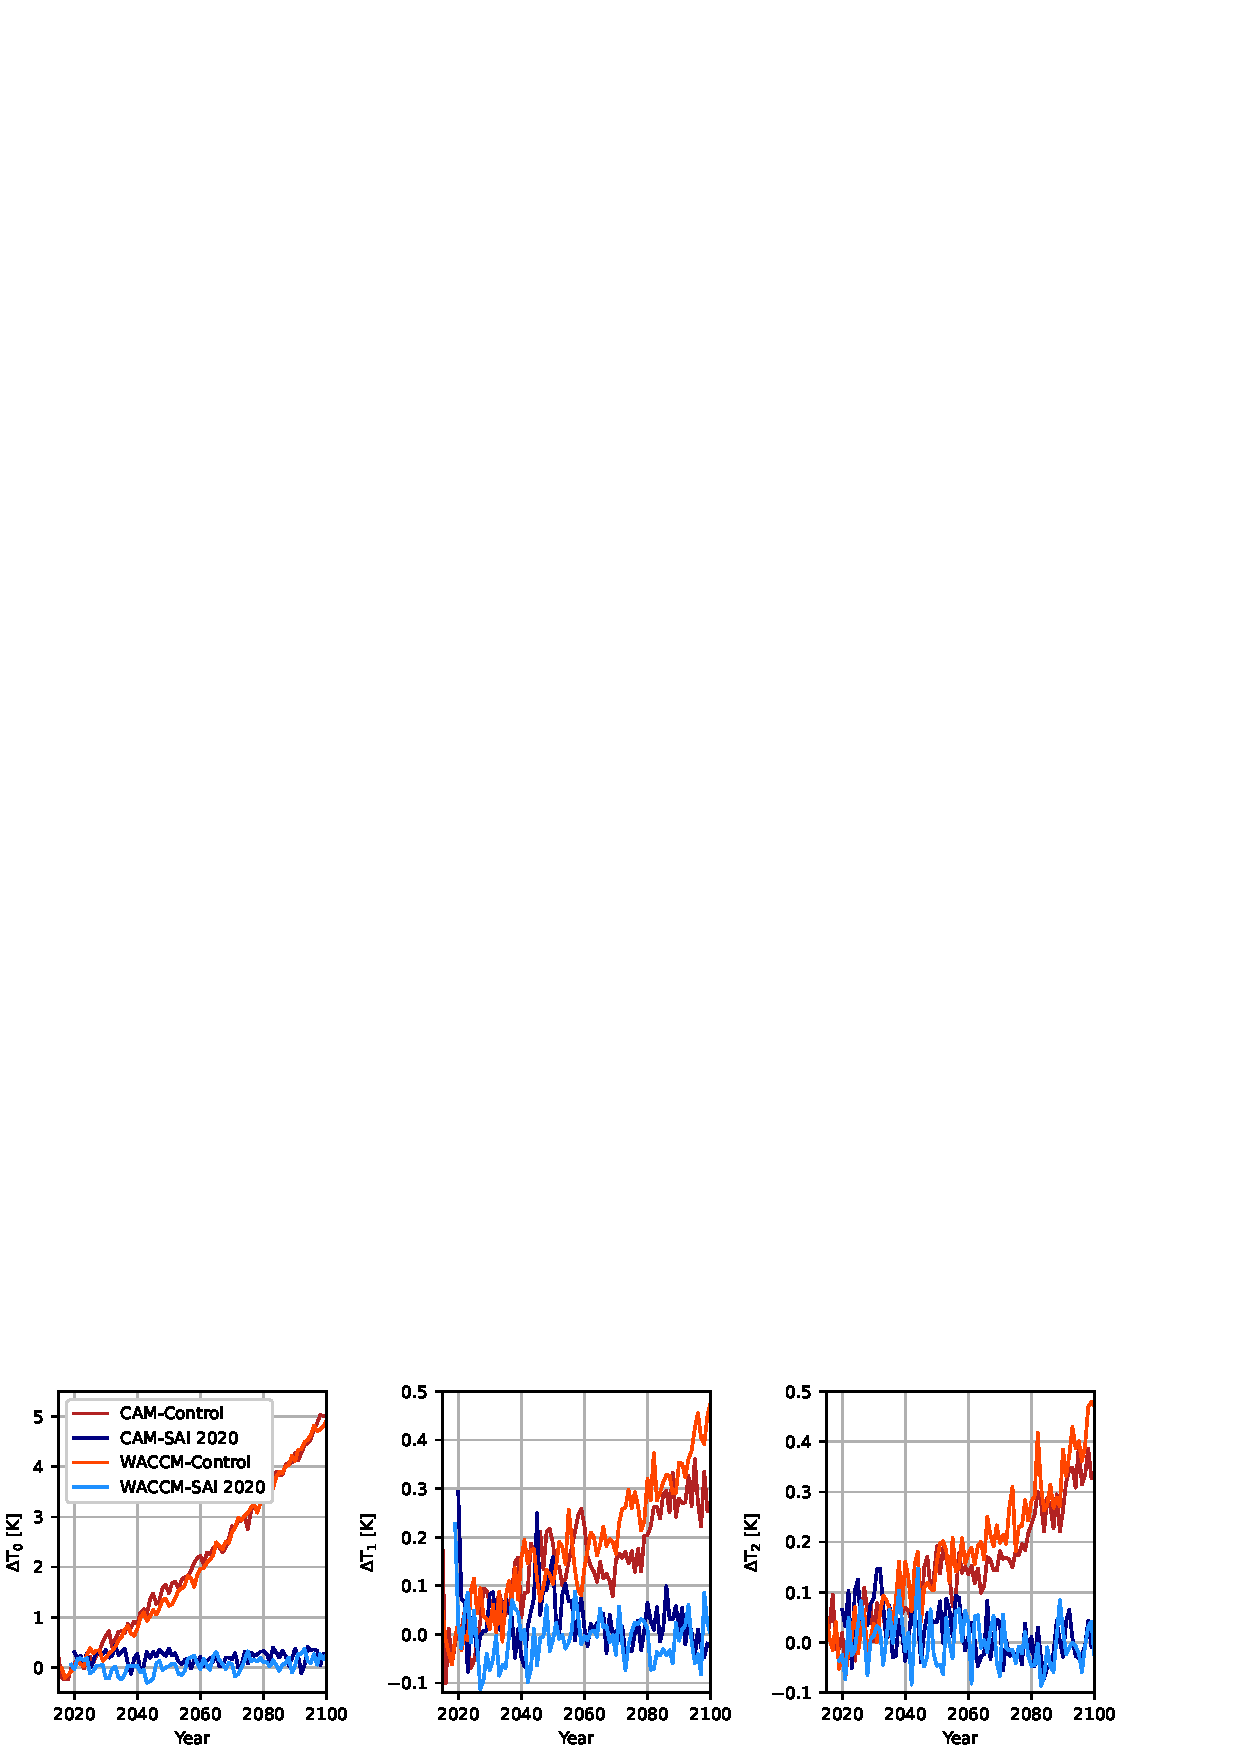
\includegraphics[width=\linewidth]{/Users/Simone/Documents/Uni/Master/Y2/Thesis/Paper_imgs/png/Tgrad_2.png}
	\caption{Temperature gradients $T_0$, $T_1$, $T_2$ as compared to 2016-2025 mean, for Control and SAI2020 scenarios in CAM and WACCM}
	\label{fig:Tgrad}
\end{figure}

The surface temperature gradients as described by Kravitz et al. are shown in Figure \ref{fig:Tgrad}, we learn:
\begin{itemize}
	\item The global mean surface temperature $T_0$ is very comparable in both scenarios between the models.
	\item Early century CAM-SAI2020 might be slightly higher, but in later century shows very similar behaviour to WACCM-SAI2020.
	\item Pole-to-pole gradient $T_1$ shows similar behaviour in the first few years, both WACCM and CAM show a clear increase compared to control after initialisation, followed by a stark drop down to reference levels. 
	\item Early-mid century CAM-SAI2020 possibly more variability compared to WACCM-SAI2020, late century very similar.
	\item -> expected because the earosol field was taken from late century.
	\item Inter-hemispheric temperature $T_2$ also shows very similar behaviour in both scenarios. 
	\item possibly more variability in early century CAM-SAI2020 compared to WACCM-SAI2020, but both seem to show a decrease in variabilty in late century. 
\end{itemize}

TO DO:
\begin{itemize}
	\item Apply some statistical analysis on these sets? Or is qualitative analasys enough? Maybe running mean and standard deviation? nah
	\item titels ipv y-labels maken 
\end{itemize}
% \subsection{Reference Height Temperature}

\subsubsection{Annual Mean Anomaly}

\begin{figure}[H]
	\centering
	\includegraphics[width=\linewidth]{/Users/Simone/Documents/Uni/Master/Y2/Thesis/Paper_imgs/png/TREFHT_ann.png}
	\caption{Annual mean reference height temperature anomalies of 2080-2099 SAI2020 scenario compared to 2016-2035 Control scenario in (a) CAM and (b) WACCM. Difference between temperature anomalies shown in (c). 2016-2035 Control mean temperature shown in black contours in 10°C intervals.}
	\label{fig:TREFHT_ann}
\end{figure}

The annual mean reference height temperature anaomalies are shown in Figure \ref{fig:TREFHT_ann}, we learn:

\begin{itemize}
	\item Spatial patterns of warming and cooling generally similar, warming over equator (especially eastern Pacific), cooling in subtropics, warming over the poles.
	\item Warming hole over North Atlantic present in both models, due to AMOC collapse in POP2 ocean model used for both CESM2 simulations. 
	\item CAM shows clear warming in the Arctic ($>$1°C), slight warming in the Antarctic ($<$1°C)
	\item WACCM only shows significant warming over Barentsz sea ($>$1°C) and similar warming over the Antarctic compared to CAM.
	\item CAM warms more than WACCM in most of the Arctic, excluding Greenland. Tropics also experience slightly more warming in CAM.
	\item CAM cools more than WACCM in Greenland/North Atlantic, North America, Northwest Pacific and Southern Ocean South of Africa. Les clearly so on Tibetan Plateau.
\end{itemize}

TO DO:
\begin{itemize}
	\item extract maximum and minimum temperature anomalies
	\item Why: difference in warming hole intensity? natural variability? of andere background conditions/fresh water fluxes form atm model
	\item Check isobars
	\item Colorbar scale - witte 0 maar hoeveel levels verder? Super custom maken?
\end{itemize}



\subsubsection{JJA and DJF Seasonal Mean Anomaly}

\begin{figure}[H]
	\centering
	\includegraphics[width=\linewidth]{/Users/Simone/Documents/Uni/Master/Y2/Thesis/Paper_imgs/png/TREFHT_seas.png}
	\caption{JJA and DJF seasonal mean reference height temperature anomalies of 2080-2099 SAI2020 scenario compared to 2016-2035 control scenario in (a),(d) CAM and (b),(e) WACCM. 2016-2035 Control mean temperature shown in black contours in 10°C intervals. Zonal mean temperature anomalies shown in (c) and (f)}
	\label{fig:TREFHT_seas}
\end{figure}

The JJA and DJF seasonal mean reference height temperature anaomalies are shown in Figure \ref{fig:TREFHT_seas}, we learn:

\begin{itemize}
	\item In \textbf{JJA} the warming hole is the largest anomaly for both CAM and WACCM, showing slight differences in intensity but overall similar extent.
	\item WACCM shows significantly more warming than CAM over the whole of the Antarctic, also represented in the zonal mean anomaly. WACCM shows slightly more warming over Western Siberia and Norhtern Canada. 
	\item CAM shows more warming than WACCM over the Eastern Pacific, mainly showing warming over an much larger extent. CAM shows slightly more warming over Alaska, Western Africa and South Asia. 
	\item in \textbf{DJF} the warming hole is still present in both CAM and WACCM, again larger extent and more intense in CAM. 
	\item WACCM shows slightly more warming than CAM in the interior of Canada/Hudson Bay and slightly more cooling over Central Asia. 
	\item CAM shows much more warming of the Arctic and Eastern Siberia than WACCM, also represented in the zonal mean anomaly. CAM shows slightly more warming over the Eastern Pacific again, as it does in JJA.
\end{itemize}

TO DO:
\begin{itemize}
	\item figure out legend for line plot.
	\item Why: much more warming over Antarctic in WACCM? Possibly ozone hole, other dynamics? 20 jaar voor 2080 ook plotten om te kijken naar natural variability.
	\item Why: warming of Eastern Pacific, due to known behaviour of ITCZ in CAM?
	\item THESIS: interannual variability meer onderzoeken voor Arctic.
\end{itemize}


\subsubsection{Annual vs. Seasonal}
When comparing Figures \ref{fig:TREFHT_ann} and \ref{fig:TREFHT_seas} we learn:

\begin{itemize}
	\item Most of the differences observed between WACCM and CAM are attributable to the winter months in the respective hemispheres. 
	\item Overall the patterns observed in the anomalies are similar, most significant differences are observed in the Arctic and Antarctic. 
	\item annual en JJA DJF samenvoegen
	\item zonal mean anomaly WACCM en CAM bundelen
\end{itemize}
% 
\subsection{Precipitation}
\subsubsection{Annual Mean Anomaly}

\begin{figure}[H]
	\centering
	\includegraphics[width=\linewidth]{/Users/Simone/Documents/Uni/Master/Y2/Thesis/Paper_imgs/png/PRECT_ann.png}
	\caption{Annual mean precipitation anomalies of 2080-2099 SAI2020 scenario compared to 2016-2035 Control scenario in (a) CAM and (b) WACCM. Difference between precipiation anomalies shown in (c). 2016-2035 Control sea level pressure shown in black contours.}
	\label{fig:PRECT_ann}
\end{figure}

The annual mean precipitation anomalies are shown in Figure \ref{fig:PRECT_ann}, we learn:

\begin{itemize}
	\item Most areas in both CAM and WACCM follow `wet gets wetter, dry gets drier'.
	\item CAM seems to have an overly active ITCZ over the pacific, though the pattern is similar to WACCM. 
	\item Southern Arabic peninsula and Horn of Africa show similar patterns, now with WACCM showing higher increase in precipitation. 
\end{itemize}

TO DO:
\begin{itemize}
	\item check slp contours/gooi ze weg, voeg reference neerslag toe
	\item min/max aanpassen? ITCZ wordt wel raar
\end{itemize}

\subsubsection{JJA and DJF Seasonal Mean Anomaly}

\begin{figure}[H]
	\centering
	\includegraphics[width=\linewidth]{/Users/Simone/Documents/Uni/Master/Y2/Thesis/Paper_imgs/png/PRECT_seas.png}
	\caption{JJA and DJF seasonal mean precipitation anomalies of 2080-2099 SAI2020 scenario compared to 2016-2035 control scenario in (a),(d) CAM and (b),(e) WACCM. 2016-2035 Control mean sea level pressure shown in black contours. Zonal mean precipitation anomalies shown in (c) and (f)}
	\label{fig:PRECT_seas}
\end{figure}

The JJA and DJF seasonal mean precipitation anomalies are shown in Figure \ref{fig:PRECT_seas} we learn:

\begin{itemize}
	\item In \textbf{JJA} the ITCZ over the pacific is again overly active in CAM, though again showing a similar pattern to WACCM. \item The higher intensity but similar pattern is also clearly visible in the zonal mean anomaly. 
	\item WACCM shows large spots of more than doubling of rainfall in Brazil and Southern Africa, not very significant still because these areas receive very little rainfall. Same goes for the increase in Australia.
	\item In \textbf{DJF} the ICTZ is even more anomalous in CAM than it is in WACCM, now not showing too similar patterns anymore, mainly not increasing in WACCM in the East Pacific. 
	\item In the Sahara region both WACCM and CAM show patches of doubling precipitation, again this is not significant as this area receives very little rainfall. 
	\item WACCM shows a more intense monsoon in Southern and South-East Asia, whereas CAM shows more limited increase in rainfall in Southern Asia. 
	\item The zonal mean anomaly shows that the Arctic is much wetter in CAM. 
\end{itemize}

TO DO:
\begin{itemize}
	\item figure out legend
	\item Why: is WACCM more sensitive for precipitation?
	\item waar regen niet significant is: arcering en/of weglaten?
\end{itemize}

% \section{Lower stratosphere wind}
% \subsection{Eddy Kinetic Energy and Zonal Mean Zonal Wind}

From Figure \ref{fig:EKE_U_zm_ann} we find:
\begin{itemize}
    \item EKE around 50°S increases in control, together with U ($\pm 5$ m/s), decreases in both SAI scenarios
    \item 
\end{itemize}

\begin{figure}[H]
    \centering
    \includegraphics[width=\linewidth]{images/EKE_U_zm_ann.png}
    \caption{Zonal mean EKE in m$^2$/s$^2$ (shading) and zonal mean zonal wind (contours) in intervals of 5 m/s, annual mean for reference 2020-2039 and all scenarios 2111-2130}
    \label{fig:EKE_U_zm_ann}
\end{figure}

\begin{figure}[H]
    \centering
    \includegraphics[width=\linewidth]{images/EKE_U_zmdiff_ann.png}
    \caption{Zonal mean difference EKE in m$^2$/s$^2$ (shading) and zonal mean difference zonal wind (contours) in intervals of 5 m/s, annual mean for reference 2020-2039 and all scenarios 2111-2130 compared to reference}
    \label{fig:EKE_U_zmdiff_ann}
\end{figure}



% \section{Polar Nigth Jet}
% From figure \ref{fig:PNJ_climatogram} we find:
\begin{itemize}
    \item temperature lower in all scenarios: stratospheric cooling from increased CO2, most significant in summer months as expected due to higher solar irradiance
    \item wind speed in ASO higher in both SAI scenarios, consistently above 100 m/s
    \item earlier development of high winds/PNJ, about 20 m/s in june compared to both reference and control
    \item occurrence of prolonged sudden stratospheric warming events decreased, as can be inferred from the lower wind speeds and higher temperatures/greater spread at the end of the season
    \item SSW's could still occur after 2100 in the simulations in all scenarios but likely of much shorter duration, thus not showin up in monthly average values
\end{itemize}
TO DO:
\begin{itemize}
    \item extend period to 30 years
    \item add 30-60°S mean T
\end{itemize}

From figure \ref{fig:PNJ_map} we find:
\begin{itemize}
    \item higher intensity for all scenarios compared to reference
    \item lower zonal wind speed in eastern pacific, WHY? compare to EKE and absolute wind speeds? appears to be no narrowing of jet
\end{itemize}
TO DO:
\begin{itemize}
    \item add gridlines (to all maps)
    \item line of maximum at 10 hPa in same figure or additional figure?
\end{itemize}

\begin{figure}[H]
    \centering
    \includegraphics[width=\linewidth]{images/PNJ_climatogram.png}
    \caption{Mean temperature $>$60°S at 10 hPa in °C and zonal mean zonal wind at 60°S and 10 hPa in m/s. Shown are reference 2020-2039 and all scenarios 2111-2130}
    \label{fig:PNJ_climatogram}
\end{figure}

\begin{figure}[H]
    \centering
    \includegraphics[width=\linewidth]{images/PNJ_map.png}
    \caption{Map of PNJ intensity above 50 hPa (?). Fractional occurence of $>$90 m/s zonal winds in each grid cell, at each model level in the months august, september and october in each time interaval. Shown are reference 2020-2039 and all scenarios 2111-2130.}
    \label{fig:PNJ_map}
\end{figure}

\begin{figure}[H]
    \centering
    \includegraphics[width=\linewidth]{images/TREFHT_ann.eps}
    \caption{Map of PNJ intensity above 50 hPa (?). Fractional occurence of $>$90 m/s zonal winds in each grid cell, at each model level in the months august, september and october in each time interaval. Shown are reference 2020-2039 and all scenarios 2111-2130.}
    \label{fig:PNJ_map}
\end{figure}



\end{document}
